\documentclass[]{dsithesis}

\usepackage{amsmath}
\usepackage{amsthm}
\usepackage{amssymb}
\usepackage{xcolor}
\usepackage{hyperref}
\usepackage{csquotes}
\usepackage{bera}
\usepackage[T1]{fontenc}

\usepackage[square,numbers]{natbib}
\bibliographystyle{abbrvnat}

\usepackage{tikz}
\usetikzlibrary{shapes,arrows,positioning}
\tikzset{sm node/.style={ellipse,fill=black!20,draw,very thick,minimum width=8cm,minimum height=5cm,inner sep=0pt},}
\tikzset{sm circ/.style={circle,fill=black!20,draw,thick,minimum width=1cm,inner sep=0pt},}
\tikzset{block/.style={rectangle,fill=red,draw,very thick,minimum width=2.5cm, minimum height=0.8cm,inner sep=0pt},align=left}
\tikzstyle{arrow} = [very thick,->,>=stealth]


\begin{document}

\author{Alexander Wagner}´

\date{TBA}
\email{wagner.2@campus.tu-berlin.de}
\course{Computer Science}
\degree{Master of Science (M. Sc.)}
\supervisorA{Prof. Dr. Florian Tschorsch}
\supervisorB{TBA: Second supervisor}

\department{Distributed Security Infrastructures}
\institute{Institut für Softwaretechnik und Theoretische Informatik}
\faculty{Fakultät Elektrotechnik und Informatik}
\university{Technische Universität Berlin}
\title{Selfish Mining and Networking Effects}
\maketitlepage
\makeatletter

\frontmatter

\newpage

\thispagestyle{empty}

\begin{large}

\vspace*{6cm}

\noindent
Hiermit erkläre ich an Eides statt, dass die vorliegende, dieser Erklärung angefügte Arbeit selbstständig und nur unter Zuhilfenahme der im Literaturverzeichnis genannten Quellen und Hilfsmittel angefertigt wurde. 
Alle Stellen der Arbeit, die anderen Werken dem Wortlaut oder dem Sinn nach
entnommen wurden, sind kenntlich gemacht. Ich reiche die Arbeit erstmals als
Prüfungsleistung ein. 
\vspace{2cm}

\noindent
Berlin, \MyDate

\vspace{3cm}

\hspace*{7cm}%
\dotfill\\
\hspace*{8.5cm}%
\textit{(\MyAuthor)}

\end{large}
	

\cleardoublepage

\chapter*{Zusammenfassung}
Bitcoin stellt die erfolgreichste Kryptowährung dar. Es setzt elektronisches Geld dezentral um. Dies wird ermöglicht durch Blockchain Technologie. Bitcoin stellt eine vielversprechende Alternative zu bestehenden elektronischen Banksystemen dar. Jedoch ist Bitcoin angreifbar. Eine zentrale Rolle in Bitcoin spielt Mining. Alternativ zum etablierten Honest Mining existieren bösartige Mining Verfahren, zum Beispiel Selfish Mining Diese ermöglichen es dem Angreifer einen Vorteil zu erwirtschaften, in dem er sogenannte Forks in der Blockchain forciert. Dies führt zu einer geringeren Growth der Blockchain und zu mehr verschwendeten Rechenresourcen. Diese Arbeit analysiert den Zusammenhang zwischen Selfish Mining und Netzwerkeffekten. Dazu nutzt sie ein neues analytisches Blockchain Modell, das sogenannte Selfish Rumor Model. Dieses Modell wird in einem diskreten Ereignis Simulator implementiert und gegenüber Blockverteilungscharakteristiken von Bitcoin validiert. Dies erzeugt zwei Parametersetups, welche genutzt werden um in einem Bitcoin ähnlichen Modell den Zusammenhang zu studieren. Es zeigt sich, dass Revenue nicht nur abhängig von relativer Rechenkraft ist, sondern auch vom Verhalten des Netzwerks. Selfish Mining ist stark davon abhängig wieviel Netzwerkvorteil der angreifende Peer besitzt. Aber auch Honest Mining kann einen erhöhten Revenue produzieren. Im Allgemeinen ist Selfish Mining in den meisten Fällen nicht profitabel. Es zeigt sich jedoch, dass das Studium divergierender Mining Strategien bisher nicht fokussierte Abhängigkeiten und Schwächen des Bitcoin protocols offenbart.

\chapter*{Abstract}
Bitcoin is the most prominent example for cryptocurrencies. It establishes a decentralized ledger utilizing blockchain technology offering a promising alternative to existent electronic cash systems. However, Bitcoin mining is vulnerable. Adversarial mining strategies such as selfish mining can be executed in order to gain an advantage. They result in a tilted incentive balance by forcing forks of the blockchain. Thus, they lower the growth of the blockchain and lead to wasted computational resources. In this thesis we analyze the relationship between selfish mining and networking effects. We study the relationship by implementing of a new analytic blockchain model, the Selfish Rumor Model. The simulator of the Selfish Rumor Model is validated against Bitcoins block propagation and establishes two parameter setups. Both parameter setups are used to study the impact of networking effects on selfish mining. We find that obtained revenue is not only linked to computational resources, but also linked to network behavior. Selfish mining is strongly influenced by the network advantage a peer possesses. However, honest mining can also produce an increased revenue.
Overall we come to the conclusion that selfish mining is not beneficial in most cases. However, exploring adversarial mining strategies and networking effects is important, since this exploration reveals certain dependencies and weaknesses of the Bitcoin protocol.


\cleardoublepage

\tableofcontents
\cleardoublepage

\mainmatter
\setlength\parindent{0pt}
\chapter{Introduction}\label{chap:introduction}
Bitcoin is the most prominent example of a decentralized cryptocurrency~\cite{1}. Before the development of Bitcoin a decentralized cryptocurrency had been envisioned for many years. It is a system, where a ledger is kept consistent among multiple parties in a peer-to-peer network without the need of trust. It enables the deployment of electronic cash without a central authority figure like a bank.
For this reason it is an enhancement to the currently established electronic banking system.

 A consistent distributed ledger is essentially a consensus problem, which has to be solved in a cooperative, distributed manner. It is therefore a Byzantine Agreement problem~\cite{garay2015bitcoin}. Bitcoin assumes an honest majority in a public system~\cite{tschorsch}. Thus, the consistence and correctness of the ledger reduces to a voting problem. However, voting in a public distributed system remains a hard problem, especially considering sybil attacks~\cite{sybil}. Bitcoin reduces the effectiveness of sybil attacks by binding voting right to computational power.
In order for a peer to participate in the system, he has to solve a cryptographic puzzle.
This process, also known as mining, consumes the computational ressources of the peer. Since there would be no reason to waste computational ressources without gain, mining is incentivized. A miner receives a so called mining reward for mining a block. This incentivized process helps spreading the overall computational power of the network among multiple different parties, since every party is competing for mining rewards.
Since mining is inherently constructed through incentives, miners will strive for the best strategy to maximize rewards. \citeauthor{eyal} show the existence of deviant mining protocols with greater rewards. Miners executing such protocols are called selfish miners. This imposes a threat, since it reduces the performance of the overall system. Additionally selfish miners obtain a greater voting power than their computational ressources allow and as a result tilt the honest majority balance.

The central goal of this master thesis is to analyze the impact of selfish mining as an attack on blockchain systems. 
While it has been established that selfish mining imposes a threat on blockchain, it remains unassessed how big the impact is. 
Additionally, selfish mining is highly influenced by networking effects. 
Therefore, in order to assess the impact of selfish mining, analysis has to be performed in a model, which also captures the underlying network.




\chapter{Related Work}\label{chap:relatedwork}
andere netzwerk analysen paper\\
andere selfish mining strategien und deren analyse etc.\\
andere currencies und selfish mining\\ 
pool mining etc. ?\\
\chapter{Model}\label{chap:model}
In order to model networking effects and selfish mining, it is essential to capture network properties in an analytic model. The model can then be used to estimate selfish mining profitability.
\citeauthor{gopalan} have introduced a new blockchain model, which captures network properties.
\section{Bitcoin Mining Fundamentals}
To understand selfish mining and its implications on network behavior it is essential to understand bitcoin mining in general.
Bitcoin utilizes proof-of-work blockchain as a distributed ledger technology.
It includes transactions into so called blocks. Blocks possess a unique ID and reference a previous block~\cite{tschorsch}. This construct builds a directed acyclic graph. The root of this tree is also called genesis block. Thus, every block directly or indirectly references the genesis block.

A correct block includes a nonce, which solves a cryptographic puzzle. The challenge is to alter the nonce until the hash of the set of transactions, the hash of the previous block and the nonce produce a partial hash collision. Essentially, the hash has to be smaller than some threshold value, which is also referred to as difficulty~\cite{tschorsch}.
Thus, Bitcoin binds block creation to the computational ressources a peer possesses, since the partial hash collision can only be solved through trial and error. The correctness of the block is easily verifiable through third parties. Thus, Bitcoin ensures a fair leader election through this process.

Bitcoin uses a peer-to-peer network to propagate the mined blocks in the system. The network is unstructured as every peer tries to maintain a minimum of eight connections and performs neighbor discovery over DNS, IRC and asking neighbors~\cite{tschorsch}. Blocks are propagated over the peer-to-peer layer through flooding.
Once a miner mines a block through solving a cryptographic puzzle, he can publish the block and receives rewards through transaction fees and mining rewards. This provides an incentive to the miner to generate as many correct blocks as possible~\cite{1}.

Consensus is established over the longest chain rule~\cite{1}. This means that the block ending the longest chain determines the state of the blockchain. This also implies that a miner only receives rewards, if his mined blocks are included in the main chain. Thus, a miner wants to produce as many correct blocks, that are part of the main chain, as possible. A protocol maximizing reward gain is thus incentive compatible.
A miner produces a relative share of blocks proportionally to his relative share of computational power of the whole network. Thus, a miner should produce a relative share of the main chain proportional to his relative share of computational power.

The original protocol, also called honest mining, assumes publishing blocks immediately after mining. Honest mining is assumed to be incentive compatible~\cite{1}. It follows that no miner can earn disproportionate rewards by deviating from the protocol.
Consequently, earning disproportionate rewards through deviation from the honest mining protocol, would disprove Bitcoin's incentive compatability claim.

\section{Original Selfish Mining Model}\label{eyalmodel}
One protocol deviation is selfish mining, which was first introduced by \citeauthor{eyal}~\cite{eyal}.
Selfish Mining is a vulnerability, which aims at increasing revenue through block withholding. The selfish miner aims at producing a greater relative share of blocks of the main chain, than the relative share of computational power of the network. Therefore, selfish mining violates Bitcoins incentive compatibility claim, as it offers a more profitable mining protocol than honest mining. This is problematic, since it not only breaks fair leader election, but also results in potentially longer confirmation times for transactions of users.
~\citeauthor{eyal} model the network over a set of miners. A miner finds a subsequent block after a time interval that is exponentially distributed~\cite{eyal}. They further define the revenue of a miner as his fraction of total blocks on the longest chain.
The selfish miner withholds mined blocks~\cite{eyal}. This selfish miner now possesses a private chain, which differs from the publicly known chain. Based on the difference between those two chains, the selfish miner performs actions. 
\begin{figure}
\begin{center}
\resizebox{.5\columnwidth}{!}{%
  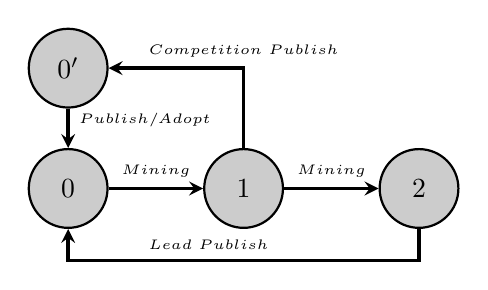
\begin{tikzpicture}
    \node[sm circ] (0) {$0$};
    \node[sm circ] (1)[right=1.2cm of 0] {$1$};
    \node[sm circ] (2)[right=1.2cm of 1] {$2$};
    \node[sm circ] (4)[above=0.5cm of 0] {$0^{\prime}$};

   	\draw [arrow] (0.east) -- node[pos= 0.5, anchor=south] {\tiny $Mining$}(1.west);
   	\draw [arrow] (1.north) |- node[pos=0.5, anchor=south] {\tiny $Competition$ $Publish$}(4.east);
   	\draw [arrow] (2.south) -- +(0,-0.4) -| node[pos=0.3, anchor=south] {\tiny $Lead$ $Publish$}(0);
   	\draw [arrow] (1.east) -- node[pos= 0.5, anchor=south] {\tiny $Mining$}(2.west);
   	\draw [arrow] (4) -- node[pos=0.3,anchor=west] {\tiny $Publish/Adopt$}(0);
   	
\end{tikzpicture}
}
\end{center}
   \caption{Abstract representation of state transtitions of eyal and sirer model for one selfish miner}
\label{fig:eyal_model}

\end{figure}
For clarification the state space and actions are modelled in Figure~\ref{fig:eyal_model}. The numbers in the states indicate the lead of the private to the public chain. $s$ denotes the lead of the private chain compared to the public chain. We can identify a total of five different actions.
\begin{itemize}
\item $Mining$: This action means that the peer has mined block. Mining adds the block to the private chain. It therefore causes $s$ to increase.
\item $Lead$ $Publish$: When $s$ increases to 2, the selfish miner will publish his private chain. It therefore causes $s$ to change from 2 to 0.
\item $Competition$ $Publish$: When $s$ is 1 and the selfish miner receives a block from another peer, he will publish his block of the same height from the private chain instead of the received one, to compete against the other miner. This causes a state transition to $0'$.
\item $Publish$: If the selfish miner is in state $0'$, he is in a competition situation.
The selfish miner will immediately publish his next mined block. This will cause the selfish miner to transition to state $0$.
\item $Adopt$: The selfish miner will adopt the main chain once he receives a new block in a competition situation.
\end{itemize}
Executing this protocol leads to a strict revenue increase, if the mining power is greater than $33\%$ according to \citeauthor{eyal}~\cite{eyal}.


\section{Gopalan Model}\label{gopalan}
The model of \citeauthor{gopalan} consists of a set of peers $P$ connected through a peer-to-peer network. Peers add blocks to the blockchain through a process called mining. 
The peer-to-peer network is modelled as an undirected Graph $H = (V,E)$.
An edge $(i,j) \in E$ represents communication possibilities between $v_i \in V$ and $v_j \in V$. 
The set of vertices is finite, such that $|V|=N \in \mathbb{N}$.
Vertices are associated with peers, such that $v_i$ represents peer $p_i \in P$.
Additionally, a directed acyclic graph $G_{p_i}(t) = (B_{G_{p_i}}(t),E_{G_{p_i}}(t))$ is associated with each peer $p_i$, at each point in time $t \in \mathbb{R+}$.
The vertex set $B_{G_{p_i}}(t) \subset \mathbb{N}$ represents the blocks known of peer $p_i$ at time $t$. The associated edge set of $E_{G_{p_i}}(t)$ represents references between blocks.
The following holds true for shorter notations:
\begin{equation}
B_G(t) = \cup_{i=1}^N B_{G_{p_i}}(t) \texttt{ and } E_G(t) = \cup_{i=1}^N E_{G_{p_i}}(t)
\end{equation}

Furthermore, the following equations hold for the principle of blockchains:
\begin{equation}
\forall p \in P: G_{p_i}(0) = (\{0\},\emptyset)
\label{genesis}
\end{equation}
\begin{equation}
t_1 < t_2 \rightarrow B_{G_{p_i}}(t_1) \subseteq B_{G_{p_i}}(t_2)
\label{nodegrow}
\end{equation}
\begin{equation}
t_1 < t_2 \rightarrow E_{G_{p_i}}(t_1) \subseteq E_{G_{p_i}}(t_2)
\label{edgegrow}
\end{equation}

Note that in this representation $0$ denotes the genesis block described in Equation~\ref{genesis}.
$G_{p_i}(t)$ evolves over time. Blocks arrive over continuous time according to a stationary point process $A$ with intensity $\lambda$. Each block $b \in \mathbb{N}$ arrives at a random peer $p_i$.
This models peer $p_i$ mining block $b$ at time $t$ and that at this time the block is also added to $B_{G_{p_i}}(t)$.
References are added to $E_{G_{p_i}}(t)$ according to policy and depending on $G_{p_i}(t^-)$, where $t^-$ is a moment in time infinitesimally before $t$. $O_i$ denotes the set of outgoing neighbors of block $i$.

The communication is modelled as a marked point process $T_{p_i}$.
Each mark corresponds to another peer $p_j \in P\backslash \{p_i\}$.
In an epoch peer $p_i$ contacts $p_j$ and thus, adds the lowest numbered block of $B_{p_i}(t)\backslash B_{p_j}(t)$ to the set of Vertices $B_{p_j}$. If $B_{p_i}(t)\backslash B_{p_j}(t)$ is not empty, $E_{p_j}$ is also updated accordingly.

The peer-to-peer network dynamics are modelled as a continuous time rumor-spreading process with exogenous arrivals~\citep{gopalan}. Since communication is bound to the process $T_{p_i}$, the block dissemination is bandwidth limited.
Reference selection and thus $O_{p_i}$ is chosen accordant to longest chain policies~\citep{gopalan}.
Let $L_{p_i}(t)$ denote the set of nodes farthest away from the genesis block $0$, known to peer $p_i$ at time $t$.
\begin{equation}
L_{p_i}(t) := \{j \in B_{p_i}(t): d(j,0)\geq d(j',0), \forall j' \in B_{p_i}(t) \}
\label{policy}
\end{equation}
Let $max\_ dist(G_{p_i}(t))$ denote that distance.
Note that the set $O_{p_i} \cap L_{p_i}(t)$ is non empty. This constructs a simple directed acyclic graph. The Tree Policy~\citep{gopalan} can then be determined as $|O_{p_i}|=1$ and establishes the following relationship:
\begin{equation}
|E_{G_{p_i}}(t)| = |B_{G_{p_i}}(t)| -1
\end{equation}
Every block will have exactly one outgoing reference, according to some deterministic rule~\citep{gopalan}. \citeauthor{gopalan} assume that the block with the lower index number will be chosen.


\section{Selfish Gopalan Model}\label{selfishmodel}
The selfish mining attack is described as a peer executing a protocol deviant from honest mining~\citep{eyal}. Therefore a selfish miner can be modelled according to the model described in Subsection~\ref{gopalan} through altering the reference selection and communication process. The reference selection process is policy driven, and can thus be modified by providing a new selfish policy. 

The first aspect to be modified is the communication process. 
Key idea of selfish mining is block withholding. The selfish miner possesses three blockchain representations. 
\begin{itemize}
\item $G_{SM_{public}}(t)$: which is updated by other peers.
\item $G_{SM_{comm}}(t)$: which is used to update other peers.
\item $G_{SM_{private}}(t)$: with the following relations:
		\begin{itemize}
		\item $G_{SM_{public}}(t)\subseteq G_{SM_{private}}(t)$.
		\item $G_{SM_{private}}(t)\backslash G_{SM_{public}}(t)$ represents blocks mined but unpublished by the selfish miner.
\end{itemize}		
\end{itemize}


\begin{figure}
\begin{center}
\resizebox{\columnwidth}{!}{%
  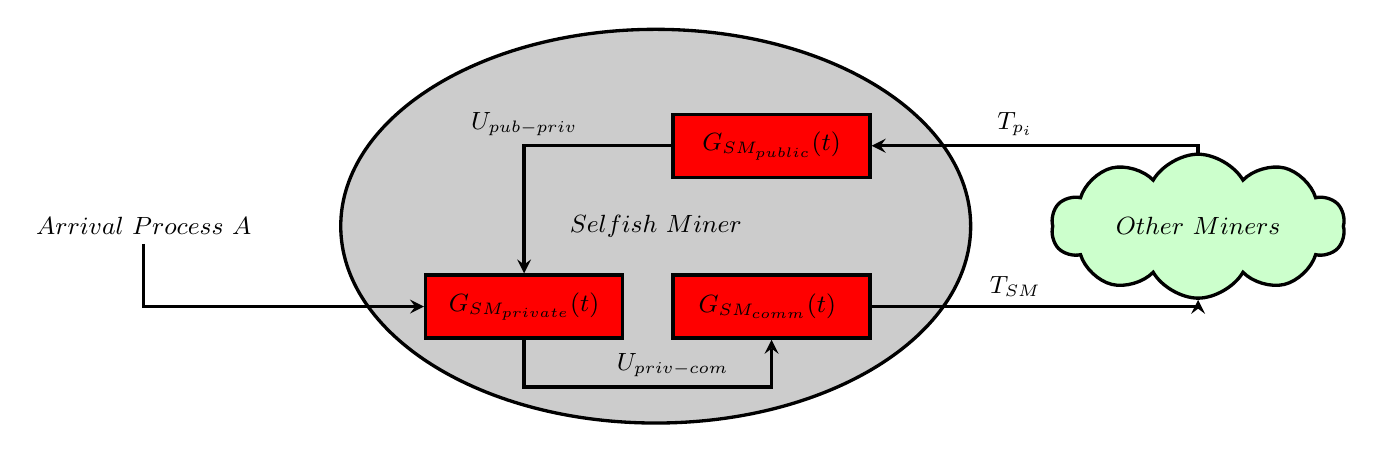
\begin{tikzpicture}
  \small
    \node[sm node] (1) {$Selfish~Miner$};
    \node(2) [left = 1cm of 1] {$Arrival~Process~A$};
    
    \node[block] (3) [above right = 0.6cm and 0.2cm]{$G_{SM_{public}}(t)$};
    \node[block] (5) [ below =1.2cm of 3 ]{ $G_{SM_{comm}}(t)$ };
	\node[block] (4) [left=0.6cm of 5]{$G_{SM_{private}}(t)$};    
    
    \node [cloud,fill=green!20, draw,very thick,cloud puffs=10,cloud puff arc=120, aspect=3, inner ysep=1em, right=1cm of 1](6) {$Other~Miners$};
    
   	
   	\draw [arrow] (2) |- (4);
   	\draw [arrow] (3) -| node[anchor=south] {$U_{pub-priv}$}(4);
   	\draw [arrow] (4.south) -- +(0,-0.6) -| node[pos=0.3, anchor=south] {$U_{priv-com}$}(5);
   	\draw [arrow] (6) |- node[pos=0.78,anchor=south] {$T_{p_i}$}(3);
	\draw [arrow] (5) -| node[pos=0.22,anchor=south] {$T_{SM}$}(6);    
\end{tikzpicture}
}
\end{center}
   \caption{Abstract representation of model entities and communication processes}
\label{fig:model_vis}

\end{figure}
The concept has been visualized in Figure~\ref{fig:model_vis}.
A total number of five processes is used to let all entities interact with each other.
\begin{itemize}
\item $Arrival~Process~A$: Blocks arrive to the selfish miner over the external arrival process $A$.

\item $T_{p_i}$: Ensures blocks from other peers are communicated to $G_{SM_{public}}(t)$.
\item $U_{pub-priv}$: Ensures that $G_{SM_{public}}(t)\subseteq G_{SM_{private}}(t)$ holds true, meaning $U_{pub-priv}$ updates $G_{SM_{private}}(t)$, when new blocks arrive to $G_{SM_{public}}(t)$ from other peers.
\item $U_{priv-com}$: Updates $G_{SM_{comm}}(t)$ according to $G_{SM_{private}}(t)$ and the selfish mining rules $S$.

\item $T_{SM}$: Ensures other peers are updated with blocks from $G_{SM_{comm}}(t)$.
\end{itemize}

Peer $SM \in P$ has an associated policy slightly different to the policy described in the gopalan model~\ref{policy}. Note that to follow the Tree Policy~\citep{gopalan}, a deterministic rule has to be established for the case that $|O_{SM} \cap L_{SM}(t)| > 1$.
Assume that $SM$ has the knowledge of the set of blocks mined through him, $M_{SM}(t) \subset B_{G_{SM}}(t)$. $SM$ will set 
\begin{equation}
(L_{SM}(t) \cap M_{SM}(t)) \neq \emptyset \rightarrow L'_{SM}(t) \subset ( L_{SM}(t) \cap M_{SM}(t)) 
\label{smpolicy}
\end{equation}
It then follows that $|L'_{SM}(t)|=1$.
This modified tree policy sets references according to the original selfish mining protocol described by \citeauthor{eyal}.

$S$ is a set of rules which describes how $G_{SM_{private}}(t)$ updates $G_{SM_{comm}}(t)$. The rules have to follow the state description of \citeauthor{eyal}~\ref{eyalmodel}. Therefore we need a state variable describing the difference between private and public chain.
Let $s$ be the state variable determining selfish mining actions~\citep{eyal}.
Then $s$ can be described as a difference between $G_{SM_{private}}(t)$ and $G_{SM_{public}}(t)$.

\begin{equation}
max\_ dist\_mined(G_{SM_{private}}(t)) := d(j,0), j \in M_{p_i}(t)
\end{equation}
\begin{equation}
s(t) := max\_ dist\_mined(G_{SM_{private}}(t)) - max\_ dist(G_{SM_{public}}(t))
\end{equation}

Let $t_{inc}$ refer to the set of times, where $s$ increased and analogous $t_{dec}$ refer to the set of times, where $s$ decreased.
Selfish mining is protocol, which needs a formulation of states in order to be characterized. \citeauthor{gopalan} introduced $t^-$ as a point in time infinitesimally before $t$. In addition to describe selfish mining a function is needed to access the point in time where $s$ changed last.
Let $f_{-1}(t)$ be a function that outputs the point in time, where $s$ changed the latest before $t$.
Now all tools are available to characterize the selfish mining protocol on top of the stochastic network model introduced by \citeauthor{gopalan}.

$U_{priv-com}$ can be characterized through four kind of update actions. Analogous to Subsection~\ref{eyalmodel}, those actions are $Lead~Publish$, $Competition~Publish$, $Publish$ and $Adopt$. $Mining$, the fifth action described in Subsection~\ref{eyalmodel}, is modelled through the arrival process.
This can be used to model the selfish mining protocol desribed by \citeauthor{eyal}.
\begin{enumerate}
\item $Lead~Publish$: Assume $t \in t_{inc}$ and $s(t) \geq 2$, then $U_{priv-com}$ updates $G_{SM_{comm}}(t)$, such that $G_{SM_{comm}}(t) = G_{SM_{private}}(t)$. Once the selfish miner has established a lead of two blocks against the public chain, he will update the blockchain representation used for communication towards other peers. In other words, he publishes the private chain.
\item $Competition~Publish$: Assume $t \in t_{dec}$, $s(t) = 0$, $s(f_{-1}(t)) = 1$, $s(f_{-1}(t)^-) = 0$. This means that the selfish miner mined a block, did not publish it and now received a block from another of the same height. This leads to the competition scenario. Accordingly, $U_{priv-com}$ updates $G_{SM_{comm}}(t)$, such that it includes the subgraph induced by the nodes on the paths between $L'_{SM}(t)$ and ${0}$. The selfish miner will publish the block, which caused the private chain to lead by one against the public chain, before he received a new block. This transitions to 
\begin{equation}
0'(t) \rightarrow \left( t \in t_{dec} \wedge s(t) = 0 \wedge s(f_{-1}(t)) = 1 \wedge s(f_{-1}(t)^-) = 0\right)
\end{equation}
This situation $0'$ is also shown and visualized in Subsection~\ref{eyalmodel} and causes the selfish miner to execute honest mining for only the next step.
\item $Publish$: Assume $0'(t^-)=\top$ and $t \in t_{inc}$, $U_{priv-com}$ updates $G_{SM_{comm}}(t)$, such that it includes the subgraph induced by the nodes on the paths between $L'_{SM}(t)$ and ${0}$. The selfish miner will publish his newly mined block, because he was previously in $0'$.
\item $Adopt$: Assume $0'(t^-)=\top$ and $s(t)=-1$, then $U_{priv-com}$ updates $G_{SM_{comm}}(t)$, such that $G_{SM_{comm}}(t) = G_{SM_{private}}(t)$. The selfish miner will adopt the public chain, because he was previously in $0'$.
\end{enumerate}
This concludes the selfish mining extension of the Gopalan Model. In the next chapters simulative analysis of this model will be focused. 









\chapter{Contribution}\label{chap:contribution}

\chapter{Evaluation}\label{chap:evaluation}
The following section utilizes the simulative implementation of the Blockchain Gossip Model to evaluate the relationship between selfish mining and networking effects. Additionally, the model will be validated against data provided by~\cauth{gopalan}~and real world data of the Bitcoin system.
\section{Simpy Blockchain Simulator}
The core implementation is based on simpy~\cite{simpy}. Simpy is a discrete event simulator written in python. As a result the Simpy Blockchain Simulator is also written in python. 
The Selfish Rumor Model consists mainly of four parts. 
\begin{itemize}
\item Networkgraph representation
\item Blockchain representation
\item Block Arrival Process representation
\item Communication Process representation
\end{itemize}
The network graph is represented by an adjacency matrix. The blockchain representation is a set of blocks and a set of edges for each peer, which are developing over time. The block arrival process and the communication process are modeled as a Poisson process~\cite{poisson}. This is mirrored in a Simpy process with an exponentially distributed interarrival time between scheduled events.
On each event of the block arrival process a block arrives at a random peer. This means that the event triggered by the block arrival process updates the blockchain datastructure accordingly.
At each event of the communication process $T_i$ a peer $p_i$ tries to update a certain peer $p_j$ according to the epoch associated with the event. This results in a comparison between the datastructures associated with $p_i$ and $p_j$ and an update of $p_j$, if it is possible.

Even though the basic implementation is simple, there are various parameters which influence the system behavior greatly. The following list shall give an overview:
\begin{itemize}
\item Average of interarrival times - This is the rate of block arrival process and communication process trigger events. 
\item Topology of the network graph - The network resulting from the adjacency matrix has a great influence on the behavior of the system.
\item Block selection - In a scenario, where multiple blocks could be transferred from one peer to another, one block has to be selected. How this block is selected influences system baviour.
\item Network size - This is the number of peers.
\item Mining power distribution - The mining power distribution influences the peer selection. Peer selection is the process of deciding which peer gets the new block once the block arrival process triggers an event.
\end{itemize}
The above discussed parameters can be modified in order to capture different systems.

\section{Validation of the Simpy Blockchain Simulator}
In the following section the Simpy Blockchain Simulator is validated against synthetic experiments published by the original authors of the blockchain gossip model. Additionally real world data from Bitcoin will be additionally used to validate the legitimacy of the Simpy Blockchain Simulator. This will lay the foundation for further analysis concerning the network and selfish mining. 
\subsection{Validation of Simulator against~\cauth{gopalan}}\label{gopalananalysis}
In the synthetic data experiments of~\cauth{gopalan}~they analyze the the network for 10, 20 and 30 peers. The network topology is a complete graph. Thus, the adjacency matrix is the unit matrix. 
The authors introduce four key metrics to analyze the system. Those are 
\begin{itemize}
\item Time to Consistency --- The average time an inconsistent system needs to reach a state of consistency
\item Cycle Length --- The sum of the average time to consistency and the average of the time the system stays consistent
\item Consistency Fraction --- The average fraction of peers that are consistent at each point in time
\item Age of Information --- The average number of blocks an average peer is away from the consistency state
\end{itemize}
All metrics mentioned above refer to the term consistency. The Consistency is defined as $B_G(t)$~\ref{unisondef}, the unison of all blocks produced by the block arrival process $A$.
In order to evaluate to capture the same system, that was analyzed by the authors, the parameters are setup similar.
These metrics can be used to verify whether the Simpy Blockchain Simulator is achieving similar numbers to the implementation of~\cauth{gopalan}. As for the parameter setup the interarrival time of the communication process is set to $1s$. The interarrival time of the block arrival process is a variable. The network topology is a complete graph. In a scenario, where multiple blocks could be transferred from one peer to another the block with the lowest index number is chosen. The network size is set to 10, 20 and 30 peers accordingly. The mining power distribution is uniform.

\begin{figure}[tbp]
	\begin{subfigure}[b]{0.5\textwidth}
		\includegraphics[width=\textwidth]{figures/gopalan_figures/time_to_consistency.png}
		\caption{ Time to Consistency}
		\label{fig:gopalan_ttc}
	\end{subfigure}
	\hfill
	\begin{subfigure}[b]{0.5\textwidth}
		\includegraphics[width=\textwidth]{figures/gopalan_figures/cycle_length_avg.png}
		\caption{ Cycle Length}
		\label{fig:gopalan_cl}
	\end{subfigure}
	\hfill
	\begin{subfigure}[b]{0.5\textwidth}
		\includegraphics[width=\textwidth]{figures/gopalan_figures/consistency_fraction.png}
		\caption{ Consistency Fraction}
		\label{fig:gopalan_cf}
	\end{subfigure}
	\hfill
	\begin{subfigure}[b]{0.5\textwidth}
		\includegraphics[width=\textwidth]{figures/gopalan_figures/age_of_information.png}
		\caption{ Age of Information}
		\label{fig:gopalan_aof}
	\end{subfigure}
	\caption{Comparison between Simpy Blockchain Simulator and values produced by~\cauth{gopalan}}
\end{figure} 

The metrics of time to consistency and cycle length are very closely related, because both rely on the time the system needs to reach consistency.
Figure~\ref{fig:gopalan_ttc} and Figure~\ref{fig:gopalan_cl} show this close relationship. Additionally the comparison between the Simpy Blockchain Simulator shows a very similar tendency in both metrics. Especially in Figure~\ref{fig:gopalan_ttc} it is observable that the curve has the same shape, only flatter. Figure~\ref{fig:gopalan_ttc} shows that peernumber and block arrival rate are proportional to the average time to consistency. Since cycle length is the sum of the average time to consistency and the average of the time the system stays consistent the same behavior can be observed in Figure~\ref{fig:gopalan_cl}. Additionally Figure~\ref{fig:gopalan_cl} shows that for very small numbers for the block arrival rate the cycle length increases again. When the system has a low block arrival rate the system tends to stay longer in a state of consistency, which is due to the fact that the idle time increases.

Consistency fraction and age of information are both metrics measuring the consistency of an average peer. The consistency fraction is the fraction of peers, which have a blockset equal to $B_G(t)$~\ref{unisondef}. For both the simulation results by~\cauth{gopalan}~and the Simpy Blockchain Simulator we can observe, that the consistency fraction decreases with an increasing blockrate and peer number. While the exact numbers do differ, similar shapes can again be observed.
The age of information metric analyzes how much an average peer differs from $B_G(t)$~\ref{unisondef}. It showcases an increase for an increasing blockrate and peer number.

The differences indicate that information spreads faster in the Simpy Blockchain Simulator. After a brief discussion with~\cauth{gopalan}, they confirmed that this might be due to the fact, that in the simpy version communication processes are handled truly concurrently.	

\subsection{Validation of Simulator against Bitcoin data}
This section validates the model against a real world blockchain system, the Bitcoin network. The Selfish Rumor Model implements an abstract network model of blockchain systems, simulating block creation and block propagation.
\cauth{neudecker-atc16} monitor the Bitcoin network and obtain data of, for example, the current block propagation delay distribution~\cite{BitcoinNetworkMonitor}. Since the model can be used to analyze blocks and their propagation, the current block propagation delay distribution is a suitable metric to compare the Selfish Rumor Model against the real world system.\\
Bitcoin block propagation has two distinct characteristics. The distribution has a high peak at around $~400ms$ and a significant long tail, with block delays going up to $30s$. Since the whole dataset contains many outliers, $5\% $ of the largest delays are filtered out. This data is then used to match parameter setups of the Selfish Rumor Model against Bitcoin and find setups offering a similar block propagation.\\
To achieve a similar block propagation one can mainly analyze the topology of the network graph and the communication process rate.
The current Bitcoin network has an unknown topology. The original protocol described an algorithm, where a peer tries to maintain at least 8 connections~\cite{tschorsch}. This would result in a random regular graph as network topology. However, analysis of the Bitcoin network comes to a different conclusion.
For example \cauth{baumann2014exploring} found strong indicators for a scale-free degree distribution.
Additionally, the FIBRE network and Compact Blocks were introduced to enable faster block propagation~\cite{measurement}. This results in a network topology, which cannot be captured by single graph representation.\\
Since the Selfish Rumor Model uses one single graph representation the objective is to utilize a topology and minimize the Root-Mean-Square-Error(RMSE). The RMSE is the standard deviation of the prediction errors~\cite{RMSE}. Since the Selfish Rumor Model Simulator can predict block propagation of Bitcoin, we can measure the error compared to Bitcoins block propagation utilizing the RMSE. Therefore, either a regular random graph or a scale free graph should be chosen as a network topology for the Selfish Rumor Model. 
\begin{figure}[tbp]
	 \begin{subfigure}[b]{0.48\textwidth}
		\includegraphics[width=\textwidth]{figures/RMSE_95.png}
		\caption{RMSE between Selfish Rumor Model regular-random Graph and Bitcoin}
		\label{fig:RMSE}
	\end{subfigure}
	\hfill
	\begin{subfigure}[b]{0.48\textwidth}
		\includegraphics[width=\textwidth]{figures/RMSE_95_barabasi.png}
		\caption{RMSE between Selfish Rumor Model scale-free Graph and Bitcoin}
		\label{fig:RMSEBar}
	\end{subfigure}
	\hfill
	\begin{subfigure}[b]{0.48\textwidth}
		\includegraphics[width=\textwidth]{figures/rmse_min.png}
		\caption{Minimum RMSE value in random-regular graph and scale-free graph}
		\label{fig:minRMSE}
	\end{subfigure}
	\hfill
	\begin{subfigure}[b]{0.48\textwidth}
		\includegraphics[width=\textwidth]{figures/propagation_histogram_withBitcoin.png}
		\caption{Selfish Rumor Model Model Block Propagation Distribution and Bitcoin}
		\label{fig:SRMBitcoin2}
	\end{subfigure}
\caption{Selfish Rumor Model Experiments in comparison with Bitcoin, 500 Peers}
\label{fig:SMRBitcoin}
\end{figure}
Figure~\ref{fig:SMRBitcoin} shows the most important results of various experiments carried out to minimize the RMSE between the simulations and Bitcoin. It also offers a comparison between the scale-free topology shown as orange and the regular random topology shown as blue. Since both topologies differ only in the degree distribution, we can compare both by their average degree respectively. All block delays were grouped in $1ms$ steps. All setups were repeated 100 times to ensure statistical significance.\\
Figure~\ref{fig:RMSE} shows the RMSE for 16, 32, 68, 100, 140 degrees and various communication process rates in comparison to Bitcoin. The lowest RMSE, $0.00016$, was achieved by 100-regular-random graph with a communication process rate of $35ms$. This parameter setup is referred to as $RegRan$. 
In Addition the results for a 16- and 32-regular-random graph are also shown in Figure~\ref{fig:RMSE}. A 32 degree regular random graph is used by~\cauth{gopalan}~to evaluate against Bitcoin data. However, the RMSE-values are significantly higher than those of the 100-regular-random graph. This is most likely due to the usage of the FIBRE relay network and Compact Blocks in Bitcoin, which decreases block propagation delay. Additionally, all curves have a clear tendency towards a specific communication rate minimizing the RMSE.\\
This is also the case for scale-free networks, as is visualized in Figure~\ref{fig:RMSEBar}. For each topology there is one minimum communication rate, minimizing the RMSE against Bitcoin block propagation delay distribution. The scale-free network is generated over the Barabasi-Albert model~\cite{BarabasiAlbert}. This algorithm has three determining parameters. The number of vertices, $m$ for the number of edges generated for each vertex and a power factor. Since the lowest RMSE was always achieved for the power factor $2$ Figure~\ref{fig:RMSEBar} shows only the RMSE for power $2$.
The lowest achieved RMSE, $0.00018$, for scale free networks was for an average of 16 m, a power factor of 2 and a communication process rate of 40ms. This parameter setup is referred to as $ScaFre$.\\
Both topologies achieve quite low RMSE values. However, Figure~\ref{fig:minRMSE} visualizes the difference between the minimum RMSE values achieved for each average degree for both random regular and scale free graphs.
Regular random graphs lower the RMSE values for an increasing average degree, until an average degree of 80. Above an average degree of 80 the RMSE values remain quite constant.\\
The analyzation of parameter setups for scale free networks is more complex. Scale-free networks, in terms of the Barabasi-Albert model, have the parameter m, which can be used to control the average degree of the network. Additionally scale-free networks have a power factor, which controls the preferential attachment process. Since 4 different power factors were analyzed for each setup, Figure~\ref{fig:minRMSE} visualizes 4 datapoints above each other for each average degree. We can observe that for $m=16$ and for $m=32$ the achieved RMSE values are the lowest for power factor 2 and a communication process rate of 40ms.\\
Figure~\ref{fig:SRMBitcoin2} visualizes the block propagation distribution from the Selfish Rumor Model for both tested topologies in their minimum configuration and Bitcoin. The regular random graph models the peak closer. The scale free network cannot model the peak as good as the regular random network, but the curve shows more distinctly the longtail behavior. The better model for lower delays achieves a better RMSE value, since lower delays contain much more data points. Since data points above 1500ms are rare for Bitcoin, the exact modelling of the long tail does not impact the RMSE value as much. Nonetheless, both parameter setups are valuable to establish a validated Selfish Rumor Model Setup.\\
We conclude this section by establishing two parameter setups. The minimum configuration for regular random networks is called $RegRan$ and the minimum configuration for scale-free networks is called $ScaFre$. Both are discussed in their differences in the above chapter exhaustively. However, there are also characteristics both share.\\
The interarrival time of the block arrival process is set to 600s. In a scenario, where multiple blocks could be transferred from one peer to another the block with the earliest arrival time is chosen. The number of peers is set to 500 and the mining power distribution is exponential. Additionally Simulations are always carried out 100 times to ensure statistical significance.\\
Those parameter setups, $RegRan$ and $ScaFre$ are used for following evaluations.

\section{Selfish Mining and Networking Effects}
Networking effects and selfish mining can be analyzed from a global and a local point of view, cf. Table~\ref{keyfactors}. The system analysis introduced by~\cauth{gopalan}~assesses the system mainly in terms of consistency and blockchain growth, as discussed in the previous section. Both, blockchain growth and consistency, are influenced by adversarial mining strategies such as selfish mining. Additionally, selfish mining is influenced by networking factors.

\subsection{Selfish Mining in homogeneous Network Setting}
\cauth{eyal} discovered a relationship between the relative computational power and the resulting $revenue~gain$. They described that an increase in networking propagation factor and relative computational power results in an increased $revenue~gain$. Additionally to the metrics of $revenue~gain$ and network propagation factor $\gamma$ we introduce two other metrics. Those are $growth$ and $forkrate$. $growth$ describes the length of the blockchain relative to the number of produced blocks and $forkrate$ describes the number of forks relative to the number of blocks~\cite{BlockPropOld}. A high $growth$ means that most produced blocks end up in the longest chain. If the $forkrate$ is significantly smaller than $1-growth$ this implies that forks tend to contain many blocks. If it is close to equal forks are mostly consisting of one block.\\
In a homogeneous network every peer has the same degree and the same bandwidth. Such a network setup is the $RegRan$ setup and it can be used to analyze selfish mining in a scenario without any networking advantage.
\begin{figure}[tbp]
	 \begin{subfigure}[b]{0.5\textwidth}
		\includegraphics[width=\textwidth]{figures/rev_and_bpr_per_peer.png}
		\caption{Revenue Gain\\ with Standard Deviation}
		\label{fig:multi_hr}
	\end{subfigure}
	\hfill
	\begin{subfigure}[b]{0.5\textwidth}
		\includegraphics[width=\textwidth]{figures/growth.png}
		\caption{Relative Average Growth of Blockchain \\with Standard Deviation}
		\label{fig:multi_hr_growth}
	\end{subfigure}
	\caption{Simulations $RegRan$ Setup, multiple Hashrates, Comparison between Peer $0$ executing honest and selfish mining}
	\label{fig:mhr}
\end{figure}
Figure~\ref{fig:multi_hr} shows the $revenue~gain$ for relative computational power between $25\% $ and $45\% $. Figure~\ref{fig:multi_hr} shows that for selfish mining the $revenue~gain$ is on average below zero except for $45\% $ relative computational power. For honest mining it is above zero. This shows that in this scenario honest mining is outperforming selfish mining. Increasing the relative computational power also increases $revenue~gain$ for the selfish miner. The small $revenue~gain$ of the honest miner increases as well, but only very slightly. The $revenue~gain$ has a greater standard deviation for the selfish miner than for the honest miner. Especially for the selfish miner $revenue~gain$ is wide spread. Nonetheless, the results contradict the \cauth{eyal} since the authors showed a strict revenue increase for $\alpha > 33\% $. Since $\alpha$ can be seen as the fraction of blocks a miner produces it is directly linked to the relative computational power this miner possesses. Thus, according to \cauth{eyal} Figure~\ref{fig:multi_hr} should be positive for the relative compuational power greater than $33\% $, which is very clearly not the case.\\
The overall $growth$ of the blockchain is influenced by the selfish mining protocol, as is visualized in \ref{fig:multi_hr_growth}. $growth$ is the length of longest chain divided by the number of produced blocks. In an ideal case the $growth$ of the blockchain is $1$ for a complete honest network. However, network effects result in a $growth$ $~93\% $ even in a total honest network. This also explains the $revenue~gain$ of the honest miner. Since the blockchain contains fork a peer producing a large amount of blocks, will gain more revenue than its relative share. We can observe as well that selfish mining lowers the overall $growth$ of the blockchain, as expected. For the setup containing the selfish miner the overall $growth$ remains constant at around $82\% $. Note, that the $growth$ reduction seems to be independent of the relative share of computational power the selfish miner possesses, at least for relative computational powers between $25-45\% $.
Selfish mining in an homogeneous network setting does not result in a $revenue~gain$ compared to honest mining.

\subsection{Selfish Mining with Network Advantage}
Selfish Mining in a homogeneous network is not beneficial. Therefore, analysis is conducted in network settings, where the selfish miner possesses a network advantage. In the following evaluations peer $0$ will possess a network advantage. This peer executes selfish and honest mining. This allows us to compare the impacts of networking advantage on honest and selfish mining. In the following experiments the selfish miner possesses a relative computational power of $45\% $.
The $RegRan$ setup utilizes a regular random graph as network topology. Increasing degree and accelerating communication process rate results in a networking advantage. 

\begin{figure}[tbp]
	 \begin{subfigure}[b]{\textwidth}
		\includegraphics[width=\textwidth]{figures/sm_edge_new_revenue.pdf}
		\caption{Revenue Gain}
		\label{fig:sm_edge_rev}
	\end{subfigure}
	\hfill
	\begin{subfigure}[b]{\textwidth}
		\includegraphics[width=\textwidth]{figures/sm_edge_new_gamma.pdf}
		\caption{Network Propagation Factor $\gamma$}
		\label{fig:sm_edge_gamma}
	\end{subfigure}
\end{figure}

\begin{figure}[tbp]
\ContinuedFloat
\begin{subfigure}[b]{\textwidth}
		\includegraphics[width=\textwidth]{figures/sm_edge_new_growth_and_forkrate.pdf}
		\caption{Growth and Forkrate}
		\label{fig:growth_fork}
	\end{subfigure}
\caption{Simulations $RegRan$ Setup with Network Advantage for honest mining(hm) and selfish mining(sm), Different Communication Process Rates Advantages}
	\label{fig:sm_edge_new}

\end{figure}
Figure~\ref{fig:sm_edge_new} visualizes experiments with network advantage. We consider Peer $0$ executing both mining strategies and alter his network parameters. The main metric to analyze mining protocols is $revenue~gain$, which is visualized in \ref{fig:sm_edge_rev}. We can observe that selfish mining results in a more spread out $revenue~gain$ than honest mining. Additionally to an increased degree the communication process rate was increased by an advantage factor, which is shown in the legend. We can observe that for almost all cases a higher advantage factor results in more $revenue~gain$. We can also observe that increasing degree does not necessarily result in an increased $revenue~gain$, in fact it may even result in a revenue loss. This is an intuitive result since in a real system splitting bandwidth between an increasing number of connections may at one point result in an overall worse performance. However, increasing both advantage factor and degree results in an overall increased $revenue~gain$.\\
Figure~\ref{fig:sm_edge_gamma} visualizes the network propagation factor $\gamma$. It is a metric only applicable to selfish mining, since it analyzes contest situation. It shows the fraction of the network receiving the selfish miner block before the contestant block. If we compare Figure~\ref{fig:sm_edge_gamma} and \ref{fig:sm_edge_rev} we observe a clear correlation between an increasing $\gamma$ and $revenue~gain$. The curve for the $5$-times advantage factor even visualizes that if $\gamma$ stagnates, the $revenue~gain$ does so as well. The $2.5$-times advantage factor curve shows at $300$ degree, that if $\gamma$ drops significantly below $50\% $, the selfish mining $revenue~gain$ drops below the honest mining $revenue~gain$.\\
Honest mining is mostly unaffected by changes in advantage factor, but very much affected by changes to the degree of the miner. However, in comparison to the $revenue~gain$ of the selfish miner the honest miner $revenue~gain$ is quite constant. The honest miner shows the highest $revenue~gain$ for a degree less than the network average. This $revenue~gain$ quickly decreases until $150$ were it starts increasing again. If we observe $growth$ and $forkrate$ in Figure~\ref{fig:growth_fork} we can see that for the degree $50$ and $100$ the $growth$ of the blockchain is the highest and constant for the honest miner scenarios. For degrees larger than $100$ the $growth$ starts rapidly decreasing. We observe the inverse behavior for the $forkrate$. Since the $forkrate$ is close to $1-growth$ the forks are very small and we can not observe a network consensus partition. For a degree greater than $150$ we can find a relationship between increasing $revenue~gain$ due to decreasing $growth$. Since the relative computational power of the miner is $45\% $ he profits from a decreased $growth$. However, the increased $revenue~gain$ for degree $50$ and $100$ with a relatively high $growth$ of $94\% $ implies that there exists a $growth$ threshold were the honest miner benefits from a better growth. We presume, that relatively more of his blocks are included in the blockchain if the growth surpasses a certain threshold.\\
The selfish miner scenarios show mostly a very similar low $growth$ and high $forkrate$. For lower advantage factors $growth$ decreases correlate to a decreased $revenue~gain$. This is most likely due to the fact, that the selfish miner can not effectively push his blocks in the main chain of the blockchain, resulting in a decreased $growth$ and increased $forkrate$.\\
However, independent of mining strategy we observe $forkrate \approx 1-growth$ which implies that for both mining strategies we only observe small forks.



















\ifx
Figure~\ref{fig:sm_edge} visualizes the results of experiments analyzing the performance of selfish mining in the $RegRan$ Setup, when the selfish miner possesses a network advantage. The network advantage was achieved by increasing degree and communication process rate of the selfish miner.
The most important metric to measure the impact of selfish mining is revenue or $revenue~gain$. Figure~\ref{fig:sm_edge_rev} visualizes revenue gain of the peer with different network advantages for both honest and selfish mining. For honest mining the revenue gain remains quite constant with any increase of network advantage. However, the smallest degree achieved the highest revenue gain. For selfish mining we observe a revenue gain for an increased networking advantage compared to honest mining. Selfish mining outperforms honest mining with more than 50 additional edges and a communication rate five times faster or more. Additionally simply increasing the communication rate can result in an increased revenue gain compared to honest mining. However simply increasing degree may also result in lowering revenue gain. Increasing degree of a peer results in a longer round robin time the peer needs to traverse all edges. This can result in a higher time for block publishing and receiving. Since fast communication is key to selfish mining, increasing degree of the selfish miner can result in suboptimal performance.
This phenomenon is also captured by Figure~\ref{fig:sm_edge_gamma}, which visualizes the network propagation factor $\gamma$. We can observe that an increase in degree without a significant increase in communication process rate results in a decreased $\gamma$. However, increasing both degree and communication process rate results in increased $\gamma$ values up to $72\% $. We can additionally observe by comparing Figure~\ref{fig:sm_edge_rev} and Figure~\ref{fig:sm_edge_gamma} that a $\gamma$ value of more than $50\% $ is correlated to a revenue gain higher than honest mining.
Figure~\ref{fig:sm_edge_growth} visualizes the growth of the blockchain. We can observe that in a system without a selfish miner the blockchain grows faster. Increasing networking advantage results in decreased growth for the honest miner. Increasing degree of the selfish miner results in decreased growth as well. However, increasing communication process rate in addition to degree for the selfish miner results in a constant growth.
\fi



\ifx
\newpage
\textcolor{red}{Ab hier, TODO}
\subsection{Selfish Mining with Networking Advantage}

topological advantage, and "bandwidth"

"trying to make selfish mining work"
\subsection{On Achievability of Networking Advantage}
betweeness centrality discussion
\subsection{Selfish Mining and Global Network Characteristics}
vllt das ans ende?	

mainly focus on growth? growth analyse war leider bisher etwas enttäuschend

This section will analyze how global system behavior changes when peers executing selfish mining are introduced to the system. In Section~\ref{gopalananalysis} the Simpy Blockchain Simulator was verified against the results published by~\cauth{gopalan}. The authors analyzed the blockchain system from a global perspective using metrices based on growth and block propagation. Thus, those base metrices will be first used to analyze the global state with adversarial miners.

\textcolor{red}{TODO: vgl. zwischen sm und nicht etc.}

Selfish mining leads to intentional forks in the blockchain.

  






\subsection{Networking effects impacting selfish mining}
Central to this thesis remains the question how impactful network effects are on the performance of selfish mining. The comparison of local and global factors from a single peer point of view can be utilized to describe a networking advantage this peer possesses.
Selfish mining is executed in order to gain revenue. Revenue gain can be measured by comparing the actual revenue to the relative computational power of the peer.
\subsubsection{Computational Power and Selfish Mining}


\subsubsection{Network Advantage and Selfish Mining}
Key aspects determining networking characteristics of a specific peer are his location relative to the network and his bandwidth, while key factors on a global scale are topology, network size and bandwidth distribution, as described in Table~\ref{keyfactors}. If for example all peers in the network possess the same amount of bandwidth, increasing the bandwidth of the selfish miner will put him at a network advantage.
If the network topology is described as a $k$-random regular graph, then allowing the selfish miner to connect to more then $k$ peers will result in a networking advantage. This topological factor can be measured by graph metrices, such as betweeness centrality.

\paragraph{Betweeness Centrality}
If revenue gain is positively correlated to network advantage, than a goal of a selfish miner should be to increase his network advantage. As discussed before one can analyze the resulting networking advantage utilizing network metrices such as betweeness centrality.
\begin{figure}[ht]
	\includegraphics[width=\textwidth]{figures/betweeness_centrality.png}
	\caption{Betweeness centrality for various k-random-regular graphs for an all-connected peer $0$}
	\label{fig:bet_cent}
\end{figure}
Figure~\ref{fig:bet_cent} visualizes the betweeness centrality of one peer in various k-random-regular graphs. This specific peer, peer $0$, is connected to all other nodes. The rest of the graph follows a random-regular structure. The x-axis visualizes the increasing $k$ of the k-random-regular graph. As $k$ increases the betweeness centrality of peer $0$ decreases. For smaller node amounts the decrease is faster than for bigger node amounts. This is due to the absolut increase in $k$ since a 20-regular-random graph of 100 peers is better connected than a 20-regular-random graph of 1100 peers. Better connected means in this case it is closer to a fully connected graph. The closer the graph gets to being fully connected the more the central role of peer $0$ decreases, since the number of alternative paths between any other two peers rises. Nonetheless, Figure~\ref{fig:bet_cent} shows the upper limit for peer $0$. This means that in general a peer has to connect to a large amount of peers, compared to the network average in order to obtain any networking advantage.

\subsubsection{Topological Networking Advantage}
It can be assumed that a peer with a higher degree than the network average possesses a networking advantage. Thus, raising the degree of the selfish miner puts him at a topological networking advantage. We can then estimate the actual networking advantage based on the betweeness centrality and $\gamma$ of the peer. 
\begin{figure}[ht]
		\includegraphics[width=\textwidth]{figures/full_sm_multi_degree_200rev_and_bpr_per_peer.png}
		
\caption{Betweeness Centrality, Revenue Gain and Network Propagation Factor, Topological Advantage Simulations with 200 Peers}
\label{fig:top_adv200}
\end{figure}

Figure~\ref{fig:top_adv200} shows results of experiments, which were based on analyzing the impact of topological network advantage. The experiments were carried out with 100, 200 and 300 peers respectively. Figure~\ref{fig:top_adv200} shows the results of the simulations for 200 peers, since no significant difference could be observed between 100, 200 and 300 peers simulations. The selfish miner possessed a relative computational power of $45\% $ while the rest was exponentially distributed on the remaining network. The interarrival time for communication process events was set to $1s$. The interarrival time for the block arrival process was set to $100s$. The selfish miner was connected to all peers. The rest of the network topology formed a $k$-random-regular graph, with an increasing $k$ shown in the x-axis.

The green bars represent the betweeness centrality of the selfish miner. The betweenness centrality of the selfish miner decreases as $k$ increases. The blue bar represents $\gamma$. We can observe that for each categroy of peer amounts $\gamma$ is slightly highest for $k \in \{0,1,2\}$ and is rather constant for $k>2$. $\gamma$  constant at around $0.55$ even though the betweeness centrality drops for increasing $k$'s. Thus, it is likely that $\gamma$ and  betweeness centrality are not correlated.

We can further observe that the revenue gain, shown in red, is highest for $k=0$. This is understandable since at $k=0$ the selfish miner can effectively eclipse every peer. The selfish miner is in total control over the information flow. For $k=1$ and $k=2$ revenue gain begins decreasing towards $0$ revenue gain. At $k=1$ and $k=2$ the selfish miner can still eclipse parts of the network but since overall connectedness increases, it becomes harder for the selfish miner to effectively eclipse every peer in the network. For $k>2$ revenue gain still seems to be slightly above $0$ which suggests that selfish mining is profitable.


\fi




















\chapter{Conclusion}\label{chap:conclusion}
In this thesis we study the relationship between selfish mining and networking effects. We evaluate the effectiveness of adversarial mining strategies in two system parameter setups validated against Bitcoin. We come to the conclusion that selfish mining is highly dependent on the network. In a setup were selfish mining is executed without network advantage it almost always outperformed by honest mining. However, if relative hashrate and network advantage are high enough selfish mining is beneficial. We find that for a relative hashrate of $45\% $ and a bandwidth 10 to 25-times faster than the average peer, selfish mining can outperform honest mining. We also observe that honest mining is dependent on relative hashrate and the network. In fact, honest mining can produce significant revenue gain with high hashrate. This gain is a result of imperfect blockchain growth, which is due to block propagation characteristics. Thus, it is reasonable to state that in most cases it is more beneficial to execute honest mining than selfish mining, unless a significant network advantage can be obtained.\\
It is up to future work to explore different adversarial mining strategies. With the astonishing performance of honest mining it might be beneficial to execute a protocol similar to honest mining, but without the obligation to propagate all blocks. If the peer has a high network influence it might be beneficial for him to exclude blocks from advertisement.\\
Overall we observe revenue gain on peers with a high relative hashrate. This implies that it is beneficial to obtain a high relative hashrate. Thus, the formation of mining pools becomes even more rewarding. However, this can lead to a reduced decentralization, if the most economically rewarding strategy is to form big mining pools. We do believe that this is not in the best interest for blockchain systems such as Bitcoin. Therefore we must explore different strategies to achieve a better growth of the blockchain.  We assume that a growth of close to 1 would reduce the revenue gain of big mining pools. The result would be a more stable decentralized cryptocurrency.

\backmatter

\cleardoublepage

\backmatter
\bibliography{references.bib}
    
\end{document}
